% Chapter 2

\chapter{Literature Review} % Introduction

\label{Chapter2} % 

Within literature the most common way of tackling the problem is through Point Processes. More recently both Gaussian Processes and Deep Learning have been applied.

\section{Point Processes}
A temporal point process \parencite{DaleyJones} is a way of modeling events data with $t$ being a sequence of a fixed period interval with $t_i \epsilon R + and i \epsilon Z+$. 

It can be modelled as a series of inter-event times (time until next event) or the number of events occurring in the interval. Examples of point processes are the times between financial transactions \parencite{EngleRusell}, and the times at which a customer makes a purchase from an online retailer *** insert ref***.

At its simplest a point process can be represented as:
$${\xi =\sum _{i=1}^{n}\delta _{X_{i}},}$$

where $\delta$ denotes the Dirac measure, a probability measure of whether a set contains point x or not.

Point processe models seek to estimate the probability of an event happening at time t, based on an event history upto, but not including, time $t$. 

There are different ways of representing point process data as shown in figure \ref{fig:fig1}, with the inter-event time being the most common. 

\begin{figure}[h!]
	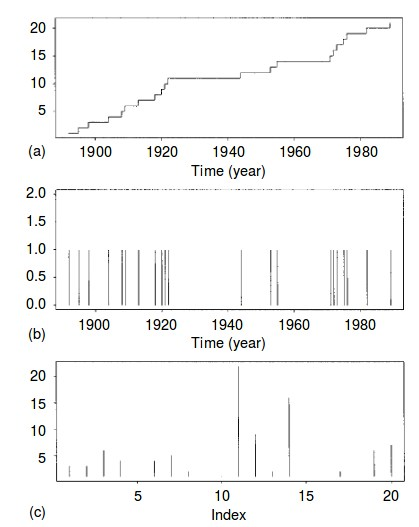
\includegraphics[width=7cm, keepaspectratio]{fig001.jpg}
	\caption{Three different representations of the same point-process a) cumulative count b) date of occurence c) interval time between floods}
	\label{fig:fig1}
\end{figure}


\subsection{Conditional Intensity Function}

A conditional intensity function is the most popular method for modeling point processes \parencite{DuWang}. In this method the probability of an event $\lambda(t)$ is derived from a stochastic model such as the Poisson process. 

Conditional intensity functions can be inhomogenous such as with a Gaussian Kernel $\lambda(t) = \sum^k_{i=1}\alpha(2\pi \sigma^2_i)^{-1/2}exp(-(t-c_i)^2/\sigma^2_i)$
, for $t \epsilon [0,T]$ where $c_i$ and $\sigma$ are fixed center and standard deviations, respectively, and $\alpha_i$ is the weight for kernel i.

Or they can vary in intensity such as with the self-exciting (Hawkes) process where the intensity is determined by previous events through the parametric form $\lambda(t) = \mu + \beta \sum_{t_i<t}g(t-t_i) where g is some non-negative kernel function.$

However, as noted by Wass et. al \parencite{Wass}, conventional point process models often make unrealistic assumptions about the generative processes of the event sequences. The conditional intensity function make various parametric assumptions about the latent dynamics governing the generation of the observed point patterns. As a consequence, model misspecification can cause significantly degraded
performance using point process models.

\section{Deep RNN Point Process Models}

In recent years deep learning has demonstrated the power to learn hierarchical nonlinear patterns on large-scale datasets \parencite{DL} through multiple layers of abstraction (e.g. multi-layer feedforward neural networks). It has achieved state-of-the-art performances on a wide range of applications, such as computer vision \parencite{ImageNet}, natural language processing \parencite{Socher}, and protein structure prediction \parencite{Lena}.

However it has not been applied to temporal point processes until recently with Xiao et. al \parencite{Wass} applying Generative Adversarial Networks (GANS) to the problem. GANs consist of two neural network models - a generator tasked with generating (i.e. predicting) a future sequence of events based on the history, and a discriminator tasked with detecting the true (fround truth) sequence amongst the generated ones.

For measuring the loss between a generated and true sequence, the authors found the Wassertein-Distance \parencite{WassGAN} performed better than Maximum Likihood Estimate (MLE) which they remarked "may suffer from mode dropping or get stuck in an inferior local minimum".

Their findings showed that where as parametric point process models work better with problems where a parametetric form exists, with real world data a GAN model with Wasserterin-Distance outperformed all other models (including an RNN model using MLE). This signals a promising new direction for temporal point process research.

